\documentclass[fleqn, a4paper, 11pt]{article}       %fleqn => flushleft equation, setzte alle Formeln linksbündig
\usepackage[ngerman]{babel}
\usepackage[utf8]{inputenc}
\usepackage[official]{eurosym}
\usepackage{amsmath}
\usepackage[onehalfspacing]{setspace}
\usepackage{booktabs}
\usepackage{siunitx}
\sisetup{locale=DE}
\sisetup{per-mode=fraction}
\usepackage{graphicx}
\usepackage{pdfpages}
\usepackage{wrapfig}
\usepackage{subfigure}
\usepackage[toc,page]{appendix}
\usepackage[left=2.5cm,right=3cm,marginpar=3cm]{geometry}
\usepackage{paralist}


%Für Zitate
\usepackage[backend=biber,style=alphabetic]{biblatex}   %evtl immer mal wieder <biber Kurzbericht_ELK1_arndt-karger.bcf > laufen lassen; \cite{tl084}

\addbibresource{literatur.bib}


\begin{document}

\begin{titlepage}
	\centering
	%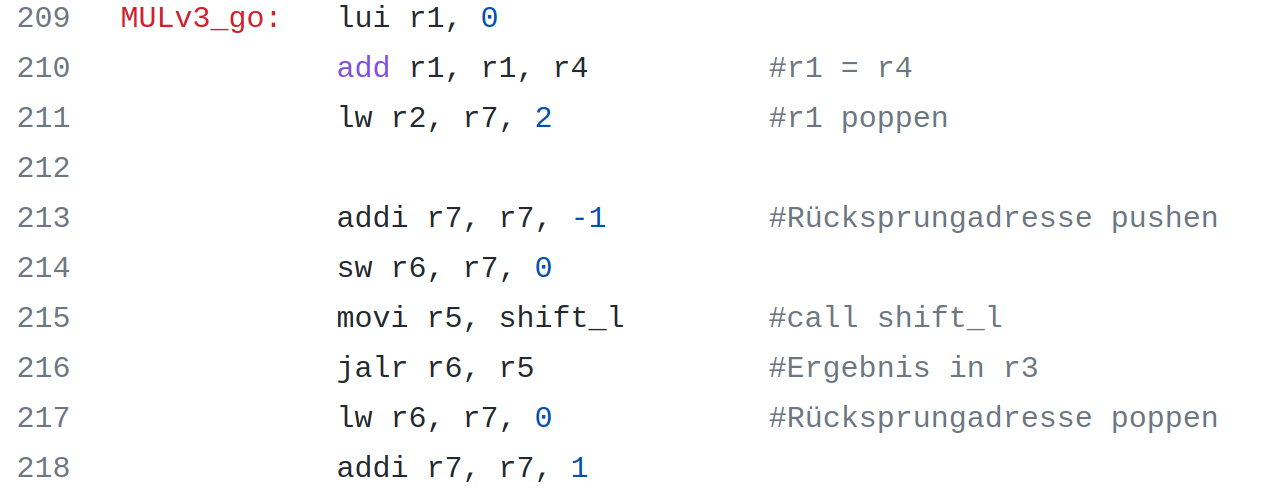
\includegraphics[width=0.8\textwidth]{Titelbild.png}\par\vspace{1cm}
	{\scshape\LARGE Technische Hochschule Mittelhessen \par}
	\vspace{1cm}
	{\huge\bfseries Dokumentation der Projektarbeit \par}
	\vspace{1.5cm}
	{\scshape\Large Systemroutinen für einen RiSC16-Prozessor \par}
	\vspace{2cm}
	{\Large\itshape vorgelegt von: \\ Arndt Karger \\ Elektro-  und Informationstechnik\\ Matrikel-Nr. 5317057\par}
	\vfill
	Betreuer:\par
    Prof. Dr.-Ing. Werner Bonath
	\vfill

% Bottom of the page
	{\large Gießen, \today\par}
\end{titlepage}

\thispagestyle{empty}
{\huge\bfseries Selbstständigkeitserklärung \par}
\vspace{1cm}

\noindent Ich versichere, dass ich die vorliegende Arbeit selbstständig verfasst und keine anderen als die angegebenen
Quellen und Hilfsmittel benutzt habe. Die Arbeit hat in gleicher oder ähnlicher Form noch keiner anderen
Hochschule oder Prüfungsstelle vorgelegen.

\vspace{4cm}
\begin{flushleft}
\begin{tabular}{@{}l@{}}\hline
Ort, Datum, Unterschrift
\end{tabular}
\end{flushleft}

\newpage
\thispagestyle{empty}
\tableofcontents
\newpage
\setcounter{page}{1}

\section{Einleitung}
Bei dem vorliegenden RiSC16-Prozessor handelt es sich um eine der MIPS-Architektur (Microprocessor without interlocked pipeline stages) \cite{MIPS} ähnlichen Architektur \cite{Ausschr}, welche über einen 16 Bit Adressraum, acht Register und acht Befehle verfügt. Des Weiteren stehen ein Assembler \cite{JACOB}, ein Simulator \cite{Bonath} sowie eine Hardwareimplementierung als FPGA (Field Programmable Gate Array) zur Verfügung. 

Es ist nicht geklärt ob die Hardwareimplementierung fehlerfrei funktioniert. Auch unklar ist die Leistungsfähigkeit der Prototypenhardware und ob umfangreiche Programme korrekt abgearbeitet werden können. Desweiteren ist der tatsächliche Programmieraufwand nicht bekannt, welcher zur Implementierung von nicht von der Architektur unterstützen Funktionen nötig ist.




\section{Aufgabenstellung}
Ziel dieser Projektarbeit war das Schreiben von Systemroutinen in Assembler, um die Funktion des Prozessors zu veranschaulichen, sowie die Hardwareimplementierung zu testen. Es sollte deutlich gemacht werden, dass auch mit einem einfachen Befehlssatz komplexe Probleme gelöst werden können. Dies wurde beispielhaft an zwei möglichen Multiplikationsalgorithmen durchgeführt. Die beiden Algorithmen stellen die Multiplikation via Addition und die bitweise Multiplikation dar. 

Zuerst wurde ein Stack in Software implementiert, um das Sichern von Registern beim Aufruf der Routinen möglich zu machen. Dann wurde für die Multiplikation via Addition ein Flussdiagramm (siehe Anhang \ref{A.MULv2}) erstellt und in Assembler implementiert. Nach einer kurzen Literaturrecherche über die genaue Funktion der bitweisen Multiplikation wurde auch hierfür ein Flussdiagramm erstellt (siehe Anhang \ref{A.MULv3}) und schließlich implementiert. Der Code wurde während der Entwicklungsphase in dem von Herrn Prof. Dr.-Ing. Bonath entwickelten Simulator fortlaufend getestet und mit der Versionsverwaltungssoftware Git getrackt.
\newpage


\section{Erstellte Routinen}
\subsection{Allgemein}
Der Befehlssatz der RiSC16-Architektur gliedert sich in zwei Befehle zur Addition (addiere Register mit Register \emph{add}, addiere Register mit Ganzzahl \emph{addi}), zwei Befehle für den Speicherzugriff (speichern \emph{sw} und laden \emph{lw}), einen Logikbefehl (\emph{nand}), einen Befehl zum Laden der oberen zehn Bits einer Ganzzahl (\emph{lui}), sowie zwei Sprungbefehlen (bedingter Sprung bei Ungleichheit \emph{bne}, Sprung zu Adresse \emph{jalr}) auf. Zusätzlich zu diesen acht Befehlen stehen im Assembler mehrere Makros zur Verfügung, von denen zwei verwendet wurden. Das eine Makro (\emph{movi}) lädt die Adresse eines Markers in ein Register. Das andere (\emph{halt}) stoppt den Programmablauf. Von den acht bereitgestellten Registern sind sieben frei verwendbar. Das erste Register (r0) beinhaltet immer den Wert $0000_{hex}$ \cite[1]{JACOBInstr}.


Die RiSC16-Architektur verfügt über keinerlei Stackoperationen. Daher wird beim Programmstart ein Stack in Software initialisiert. Das Register r7 dient hierbei als Stackpointer (SP). Dieses wird zuerst mit der Startadresse des Stacks (hier $7FFF_{hex}$) beschrieben. Dieser Wert steht hart im Speicher und wird über den Marker \glqq Stack\_adr\grqq \ abgerufen (siehe  Abbildung \ref{fig:Stack}).
Der Stack wurde   Bottom-Up implementiert. Dies bedeutet, dass er zu kleiner werdenden Adressen hin wächst. Das Register r7 zeigt immer auf den Top-Of-Stack (TOS). Das heißt der SP zeigt immer auf das zuletzt abgelegte Element. Die Größe des Stacks (hier 64 Zeilen) ist rein hardwareabhängig, die Grenzen des Stacks werden nicht überwacht.

Die Funktion \emph{push}  wird durch einmaliges dekrementieren des SPs und speichern eines Registers mit dem Befehl \emph{sw} (store word) erreicht (siehe Abbildung \ref{fig:Stack} line 12 folgende). Analog wird die Funktion \emph{pop} durch das Laden eines Werts aus dem Speicher via \emph{lw} (load word) und anschließendem inkrementieren des SPs erreicht. Eine indirekte Adressierung ist mittels eines Immediate-Offsets möglich (siehe Abbildung \ref{fig:Stack} line 14).

Prinzipiell ist das ausreichend, um mit dem Stack arbeiten zu können. Um eine bessere Lesbarkeit beim Debuggen zu schaffen, werden in der Initialisierung noch der Anfang sowie das Ende des Stacks markiert. Dazu wird in das Register r1 der Wert $-1_{dez}\ \widehat{=}\ FFFF_{hex}$ geschrieben und an die erste und letzte Adresse im Stack gepusht (siehe Abbildung \ref{fig:Stack} line 11 fort folgende).

\begin{figure}[h]
    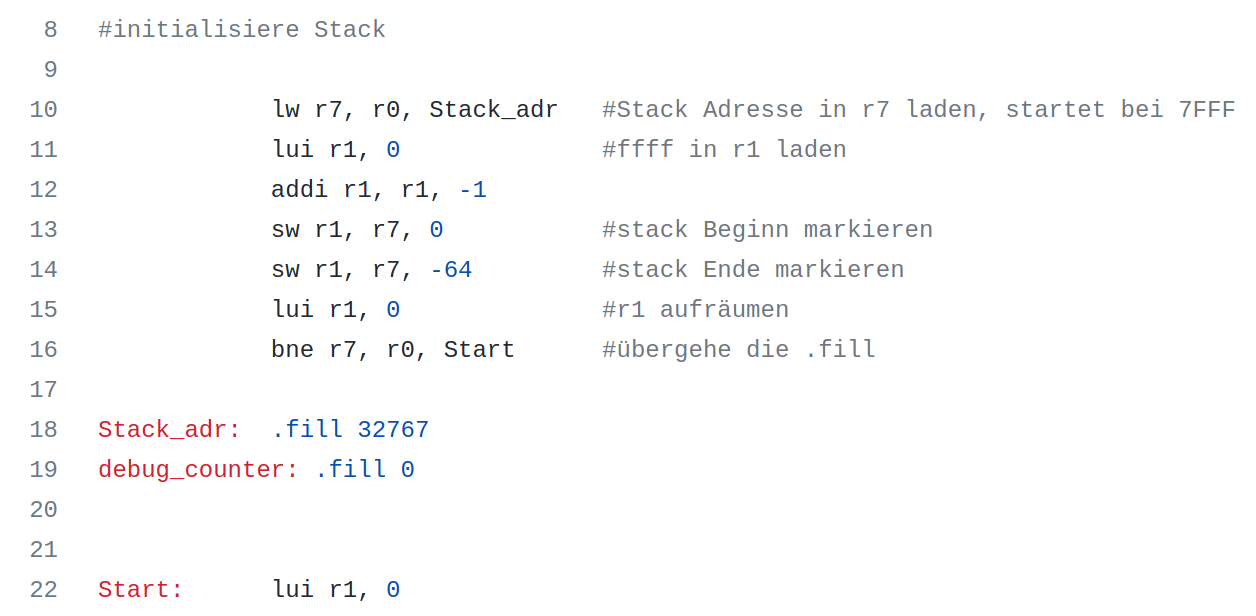
\includegraphics[width =0.9\textwidth]{Stack_init.png}
\caption{Initialisierung des Stacks}
\label{fig:Stack}
\end{figure}

\newpage
\noindent Des Weiteren wurde eine Übergabekonvention erarbeitet, die folgendes vorsieht: Es können bis zu zwei Werte an Unterprogramme übergeben werden. Diese müssen vor Aufruf des Unterprogramms in die Register r1 und r2 geladen werden (siehe Abbildung \ref{fig:FKT} line 39 folgende). Das Unterprogramm hat die Aufgabe sicherzustellen, dass nach dem Rücksprung die Registerinhalte der beiden Übergaberegister unverändert bleiben. Der Rückgabewert wird im Register r3 zurückgegeben (siehe Anhang \ref{A.Man}).

Der eigentliche Programmaufruf erfolgt über das Makro \emph{movi}. Dieses lädt die Adresse eines Markers in ein angebenenes Register, hier r5 (siehe Abbildung \ref{fig:FKT} line 43). Im Anschluss erfolgt ein Sprung durch den Befehl \emph{jalr} zu der Adresse aus r5. Die Rücksprungadresse wird in r6 abgelegt (siehe Abbildung \ref{fig:FKT} line 44).

\begin{figure}[h]
    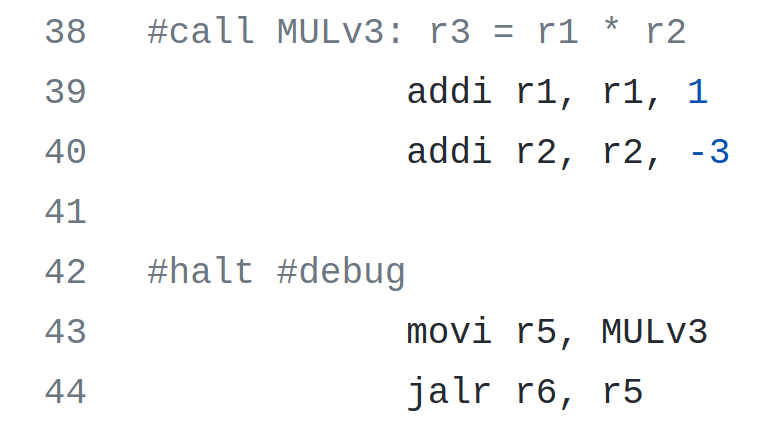
\includegraphics[width =0.4\textwidth]{Funktionsaufruf.png}
\caption{Aufruf des Unterprogramms MULv3}
\label{fig:FKT}
\end{figure}


\subsection{Multiplikation via Addition}
Eine Möglichkeit eine Multiplikation zu implementieren besteht darin, den Multiplikanten so oft zu sich selbst dazu zu addieren, wie es der Multiplikator vorschreibt. Aus $X = 3 \cdot 3$ wird  $X = 3+3+3$. Diese Art der Multiplikation ist sehr einfach durch eine Schleife zu realisieren und wurde in der Routine \emph{MULv2} angewendet (siehe Anhang \ref{A.MULv2}). Hierbei wird der Multiplikant (r2) solange auf das Ergebnisregister (r3) addiert, bis der Multiplikator (r1) zu Null geworden ist. Eine vorzeichenbehaftete Multiplikation ist nicht vorgesehen, ist jedoch prinzipiell möglich solange nur der Multiplikant negativ ist.

\subsection{Bitweise Multiplikation}
Eine andere Möglichkeit der Multiplikation besteht darin, zwei Zahlen bitweise zu multiplizieren. Der entwickelte Multiplikationsalgorithmus funktioniert nach folgendem Prinzip: 

Beispielhaft wird im Nachfolgenden die Multiplikation von zwei Acht-Bit-Zahlen \\ ($n = 8$) betrachtet. Davon ist eine Zahl der Multiplikant und die Andere der Multiplikator. Zuerst wird das Most Significant Bit (MSB), das siebte Bit, des Multiplikators (r2) untersucht. Ist dieses gesetzt, so wird der Multiplikant (r1) um die Wertigkeit des untersuchten Bits, im ersten Schritt siebenmal, nach links geschoben und auf das Ergebnisregister (r3) addiert. Ist das MSB nicht gesetzt, so wird die Addition nicht ausgeführt. \cite{MULv3}

Analog verfahren wir mit allen weiteren Bits. Diesen Prozess müssen wir für alle Bits des Multiplikators durchführen, in unserem Beispiel ergibt das acht Wiederholungen (siehe Abbildung \ref{fig:bitw_Mul_Prinzip}). Dieser Prozess ist unabhängig von der Bitbreite, da diese lediglich die Anzahl der Wiederholungen des Algorithmus vorschreibt.



\begin{figure}[h]
    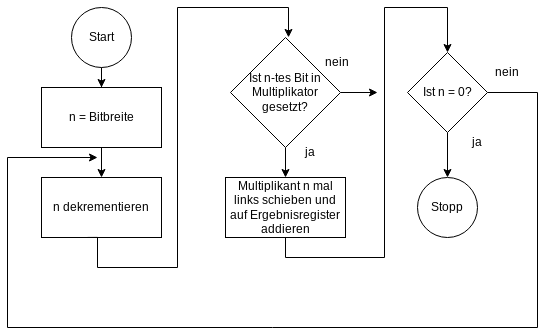
\includegraphics[width =0.8\textwidth]{bitweise_Mul_Prinzip.png}
\caption{Funktionsprinzip der bitweisen Multiplikation}
\label{fig:bitw_Mul_Prinzip}
\end{figure}



Da die RiSC16-Architektur über keinerlei Schiebebefehle verfügt, wurde hierfür ein Unterprogramm entworfen, welches als Rückgabewert das um eine gewünschte Schrittweite geschobenes Register hat und nach folgendem Prinzip arbeitet:

Im einfachen Binärsystem hat die Stelle $n+1$ immer genau die doppelte Wertigkeit der Stelle $n$, zum Beispiel $2^2 = 4 = 2 \cdot 2^1$. Wird ein Wort nach links geschoben und  rechts mit Nullen aufgefüllt, so verdoppelt sich die Wertigkeit des Wortes mit jedem Schiebevorgang. Dies kommt einer Multiplikation mit Zwei gleich. Bei einer gewünschten Schrittweite $m$ verdoppelt dieses Unterprogramm das Register  $m$-mal.

Zuletzt wurde der bitweisen Multiplikation noch ein Sortieralgorithmus vorgeschaltet, welcher automatisch die richtige Registerkonfiguration für vorzeichenbehaftete Zahlen vornimmt. Der Algorithmus untersucht die Vorzeichen (MSBs) von Multiplikator und Multiplikant. Ist genau einer der Beiden negativ, stellt der Algorithmus sicher, dass dieser im Register r1 steht (siehe Anhang \ref{A.MULv3}). 

\noindent Ein Grund für die Notwendigkeit dieser Konfiguration ist, dass ein gesetztes MSB keine Wertigkeit in einer negativen  Zahl repräsentiert, sondern nur ein Vorzeichen. Die Bits des Multiplikators (r2) werden jedoch zur Entscheidung, ob der Multiplikant (r1) geschoben werden muss, verwendet. Das bedeutet, sie werden alle als Bits mit einer Wertigkeit interpretiert. Ein Vorzeichenbit führt hier zu falschen Ergebnissen. Mathematisch sind Multiplikator und Multiplikant vertauschbar.

Analog dazu macht der Sortieralgorithmus bei der Multiplikation von zwei vorzeichenbehafteten Zahlen (beide MSBs gesetzt) die Zweierkomplementumwandlung, welche hier zur Darstellung von negativen Zahlen verwendet wird, rückgängig. Es entstehen zwei positive Zahlen (siehe Anhang \ref{A.MULv3}). Grundlage dafür ist dieselbe, oben erklärte Problematik. Mathematisch betrachtet entsteht hier wieder kein Unterschied.
\newpage
\section{Zusammenfassung}
Der Befehlssatz der RiSC16-Architektur umfasst nur acht Befehle. Damit sind die Operationen prinzipiell auf Additionen, \emph{NAND}-Logikoperationen und Speicherzugriffe beschänkt. Das direkte Arbeiten mit Speicherzugriffen und die Möglichkeit mittels Logikoperationen  einzelne Bits zu manipulieren ergibt bei der Programmierung viele Freiheitsgrade und erlaubt abstrakte Lösungsansätze. Das zeigt der Algorithmus zur bitweisen Multiplikation besonders deutlich. Der Programmumfang schwankt dabei stark zwischen etwa 30 Zeilen für die Multiplikation via Addition und 150 Zeilen für die bitweise Multiplikation. 

Tatsächliche Hardwaretests konnten in dieser Arbeit nicht durchgeführt werden. Daher stehen keinerlei  Messergebnisse zu Durchlaufzeiten verschiedener Programme zur Verfügung.

Alles in allem wird in dieser Projektarbeit deutlich, dass auch mit einem minimalen Befehlssatz praktische Problemstellungen  durch die Verflechtung verschiedener Algorithmen lösbar sind. Nicht von der Architektur gegebene Funktionen können in Software implementiert und zur Bearbeitung komplexer Problematiken kombiniert werden.

%Alte Zusammenfassung:
% \section{Zusammenfassung}
% 
% Der Befehlssatz der RiSC16-Architektur umfasst nur acht Befehle. Die eigene Implementierung des Stacks sowie der Multiplikationsalgorithmen machen ersichtlich, dass auch Funktionen, die nicht von Beginn an im Befehlssatz enthalten sind, schnell generiert werden können. Am Beispiel des Stacks sowie des Unterprogrammaufrufes wird die interne Funktionsweise des RiSC16-Prozessors deutlich.
% 
% Die Multiplikation via Addition war sehr einfach zu implementieren und benötigte nur wenige Programmzeilen. Ihre Durchlaufzeit bleibt jedoch abhängig vom Betrag des Multiplikators. Sie kann also nicht vorausgesehen werden. Dagegen ist die Durchlaufzeit der bitweisen Multiplikation nur abhängig von der verwendeten Bitbreite und somit immer konstant. Der Algorithmus der bitweisen Multiplikation war jedoch deutlich komplexer und benötigte wesentlich mehr Programmzeilen. Inwiefern sich die Durchlaufzeiten von bitweiser Multiplikation und Multiplikation via Addition unterscheiden wurde in dieser Arbeit nicht betrachtet.
% 
% Bei der Betrachtung der verschiedenen Flussdiagramme fällt auf, dass die Algorithmen schnell komplex werden. Es hat sich jedoch gezeigt, dass auch diese Algorithmen mit dem einfachen Befehlssatz der RiSC16-Architektur gut lösbar sind. In einem weiteren Schritt kann der Multiplikation via Addition analog zur bitweisen Multiplikation ein Sortieralgorithmus vorgeschaltet werden, um eine vorzeichenbehaftete Multiplikation möglich zu machen. Des Weiteren kann ein Divisionsalgorithmus entworfen werden. Hierfür wird in erster Linie eine Rechtsschieben-Funktion benötigt.



% \section{Verwendete Abkürzungen}
% \subsection{Allgemeine Abkürzungen}
% \begin{compactitem}
%     \item Abbildung : Abbildung
%     \item Bsp. : Beispiel
%     \item f. : folgende. Bsp.: line 12f. bedeutet line 12 und 13
%     \item ff. : fortfolgende. Bsp.: line 12ff. bedeutet line 12 bis zum Ende des Blocks
%     \item Vgl. : vergleiche
% \end{compactitem}
%
% \subsection{Technische Abkürzungen}
% \begin{compactitem}
%    % \item LSB : Least Significant Bit
%     \item MSB : Most Significant Bit
%     \item SP : Stackpointer
%     \item TOS : Top-Of-Stack
% \end{compactitem}

\newpage
\appendix %sagt ab hier ist Anhang
\section{Anhang}
\subsection{Verwendung der entworfenen Routinen \label{A.Man}}



 \textbf{Registerverwendung:}
 \begin{compactitem}
     \item r1: zur Wertübergabe, nach Unterprogrammaufruf unverändert
     \item r2: zur Wertübergabe, nach Unterprogrammaufruf unverändert
     \item r3: Ergebnisregister
     \item r4: Zählregister innerhalb von Funktionen
     \item r5: don't-care
     \item r6: Rücksprungadressen
     \item r7: Stackpointer
 \end{compactitem}
 \vspace{0.25cm}
 \noindent \textbf{Funktionsaufruf:}
     Definiere r5, r6 für Programmaufrufe
     \begin{compactenum}
     \item Adresse von Unterprogramm in r5 laden:\\
         \emph{movi r5, Unterprogramm}
     \item Zur Adresse in r5 springen, Rücksprungadresse in r6 speichern:\\
         \emph{jalr r6, r5}
     \item zurückspringen: (Hier ist die Rücksprungadresse (r5) unwichtig)\\
         \emph{jalr r5, r6 }
     \end{compactenum}
     
\vspace{0.25cm}
      
 \noindent \textbf{Stack:}
     Definiere SP als r7
     \begin{compactitem}
         \item push:
         \begin {compactitem}
                  \item \emph{addi r7, r7, -1}           (SP dekrementieren)
                   \item \emph{sw  r1, r7, 0 }            (r1 pushen)
           \end{compactitem}         
         \item pop:
             \begin{compactitem}
                   \item \emph{lw r3, r7, 0 }             (in r3 poppen) 
                   \item \emph{addi r7, r7, 1  }          (SP inkrementieren, damit SP immer auf letztes Ereignis zeigt)
             \end{compactitem}                                 
         \end{compactitem}  
 
  \vspace{0.2cm}

 \noindent \textbf{shift\_l:}
 \begin{compactitem}
     \item shiftweite (n) in r1, zu shiftendes Wort (a) in r2
     \item Ergebnis wird in r3 zurückgegeben
     \end{compactitem}
  
   \vspace{0.25cm}

 \noindent \textbf{MULv2:}  (MUL via add)
 \begin{compactitem}
     \item Multiplikator in r1, Multiplikant in r2
     \item Ergebnis wird in r3 zurückgegeben
     \end{compactitem}
   
    \vspace{0.25cm}

 \noindent \textbf{MULv3:}  (bitweise MUL)
 \begin{compactitem}
     \item Multiplikant in r1, Multiplikator in r2
     \item Ergebnis wird in r3 zurückgegeben
     \end{compactitem}


\newpage

\subsection{Multiplikation via Addition: (MULv2)\label{A.MULv2}}
Funktionalität: 

Multipliziere zwei vorzeichenlose Zahlen.
\vspace{0.25cm}

\noindent Verwendung:
\begin{compactitem}
    \item $r3 = r1 \cdot r2$
	\item Multiplikator und Multiplikant vor Programmaufruf  in r1  und r2 laden.
	\item Diese stehen auch nach Programmablauf unverändert   dort.
\end{compactitem}
\vspace{0.25cm}
\noindent Flussdiagramm siehe nächste Seite.

\thispagestyle{empty}
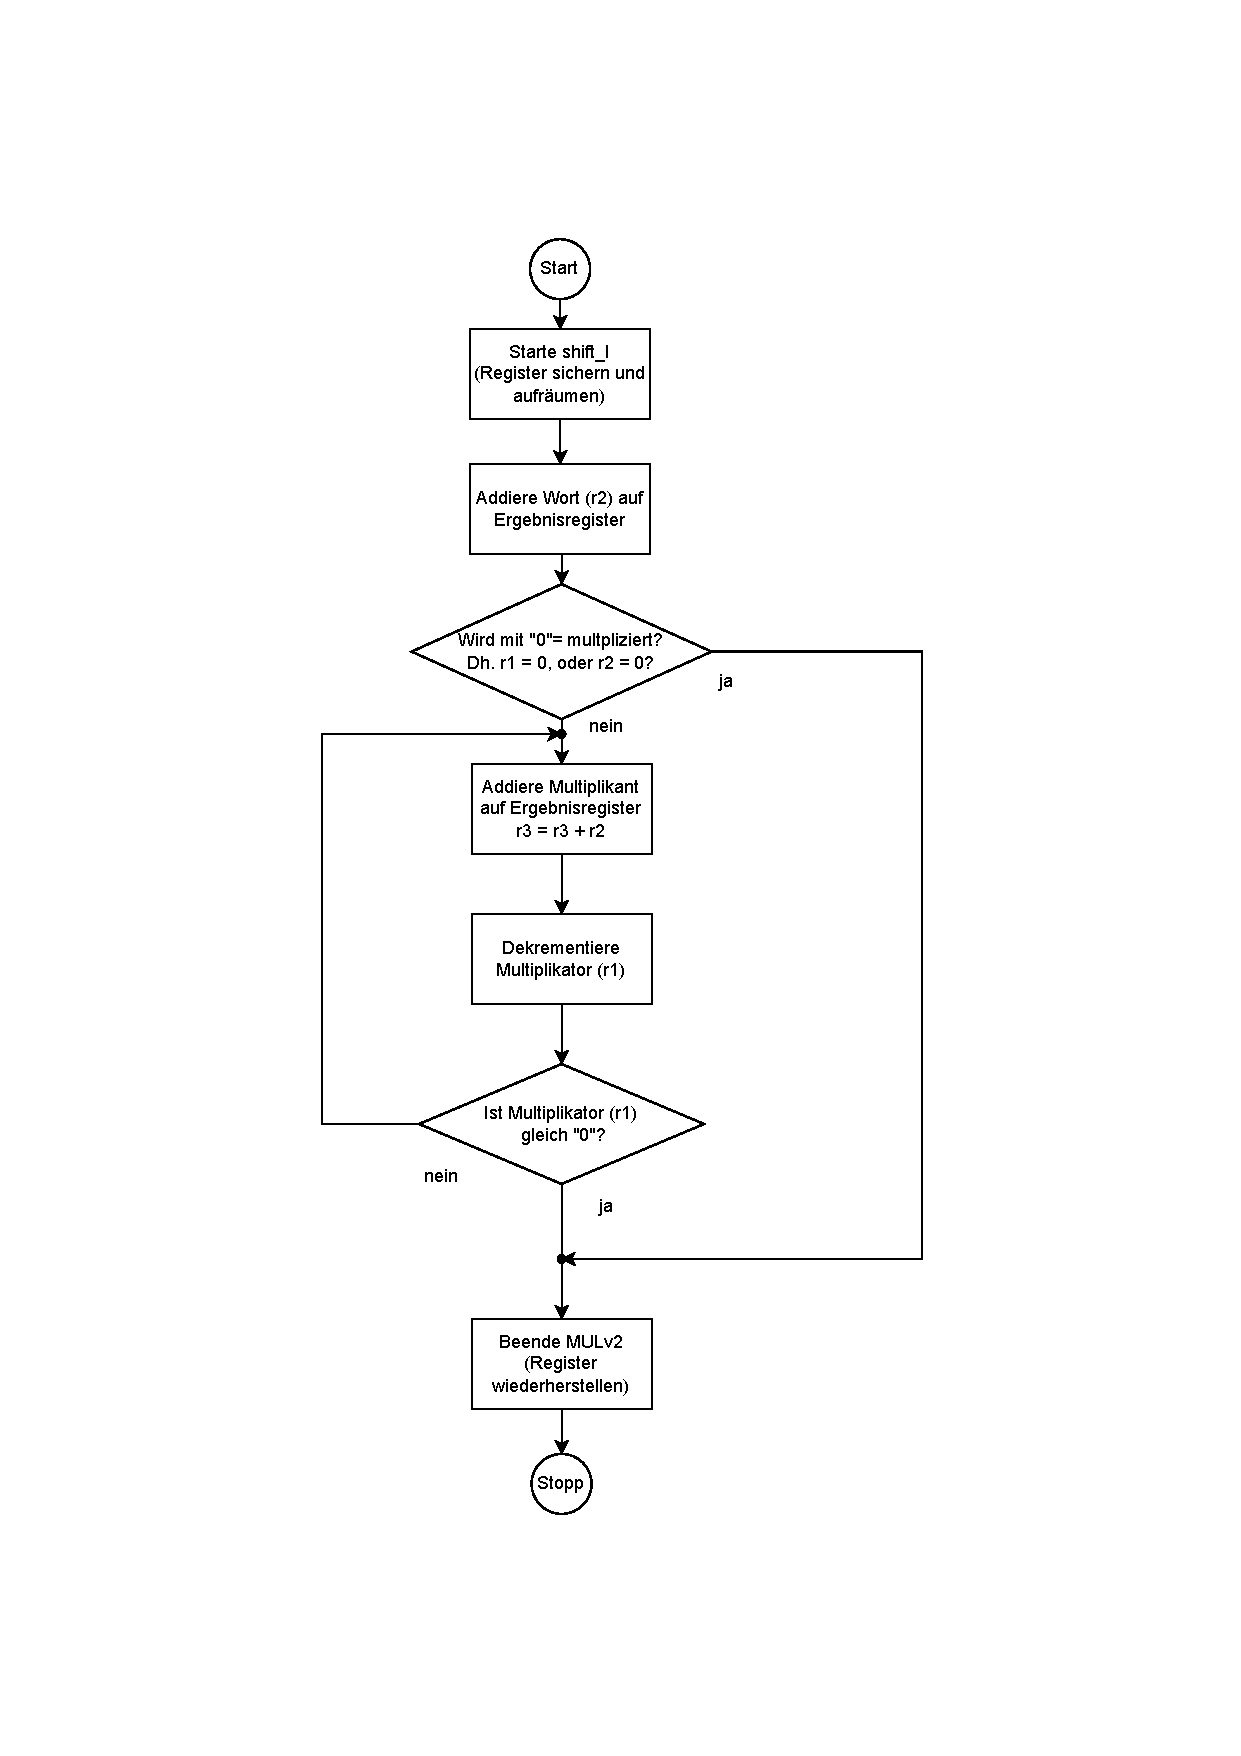
\includepdf[pages=1]{MULv2.pdf}

\newpage

\subsection{Bitweise Multiplikation: (MULv3)\label{A.MULv3}}
Funktionalität:

Multipliziere zwei vorzeichenbehaftete Acht-Bit-Zahlen.
\vspace{0.25cm}

\noindent Verwendung:
\begin{compactitem}
	\item $r3 = r1 \cdot r2$
	\item Multiplikant und Multiplikator vor Programmaufruf in r1 und r2 laden.
	\item Diese stehen auch nach Programmablauf unverändert                dort.
\end{compactitem}
\vspace{0.25cm}
\noindent Flussdiagramm siehe nächste Seite.




\thispagestyle{empty}
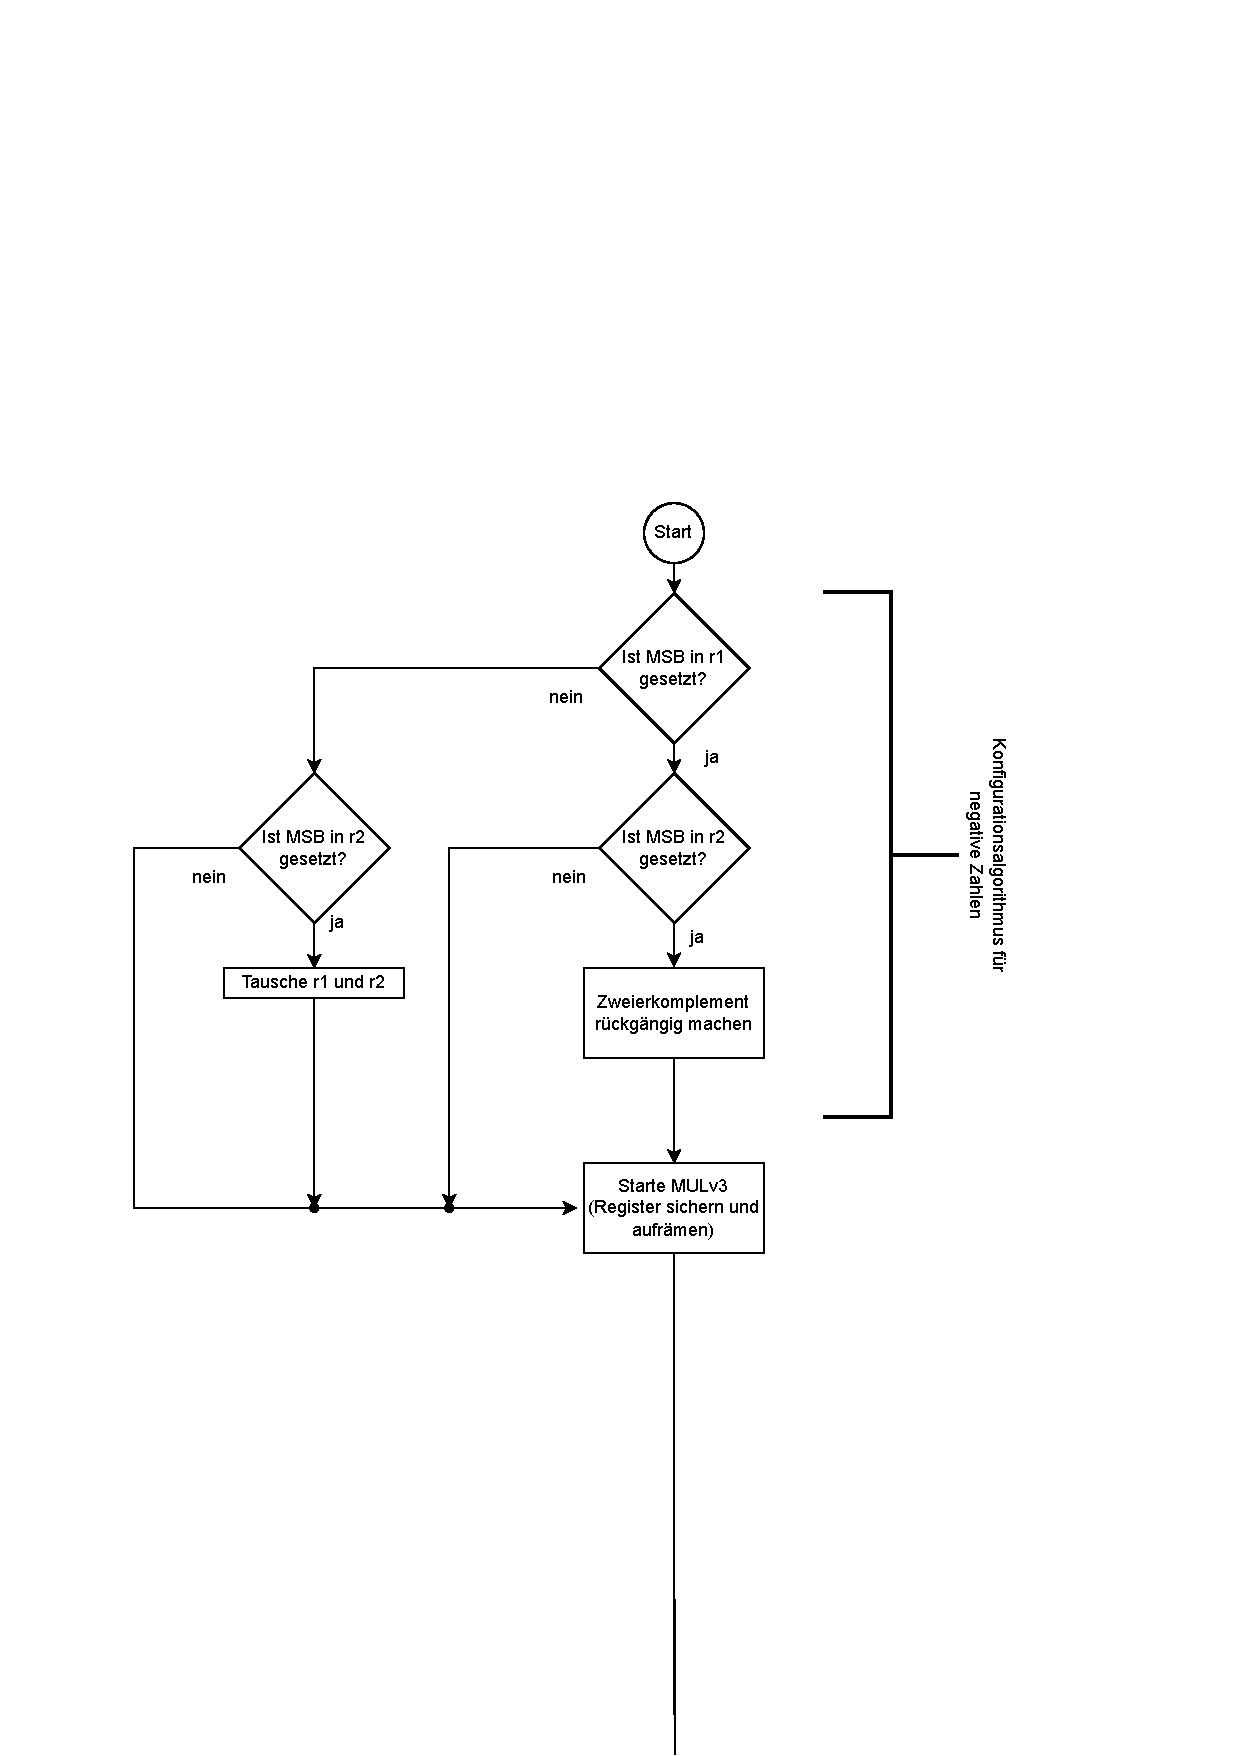
\includepdf[pages=1]{MULv3.pdf}

\thispagestyle{empty}
\includepdf[pages=2]{MULv3.pdf}





\newpage

\printbibliography  % so werden Zitate angegeben: \cite{name}
\addcontentsline{toc}{section}{Literaturverzeichnis}



\end{document}

